\section{Introducción}
  
\subsection*{Contexto}
% Una subsection* crea un nuevo "grupo de puntos"

\frame{
	\ifdebug
	\frametitle{Descripción del problema\hfill{\color{red} \emph{A}}}

	\else
		\frametitle{Descripción del problema}
	\fi

	\textbf{Objetivo}
	\vspace{0.25cm}
	\begin{center}
		“Diseñar, ensamblar y programar una planta móvil de control de 
		  nivel, utilizando sensores, controladores y actuadores 
		  industriales disponibles en el mercado”
	\end{center}
	\textbf{Es decir, algo así}...
	\begin{center}
	  %\vspace{0.25cm}
	  \begin{figure}[h!]
	  \centering
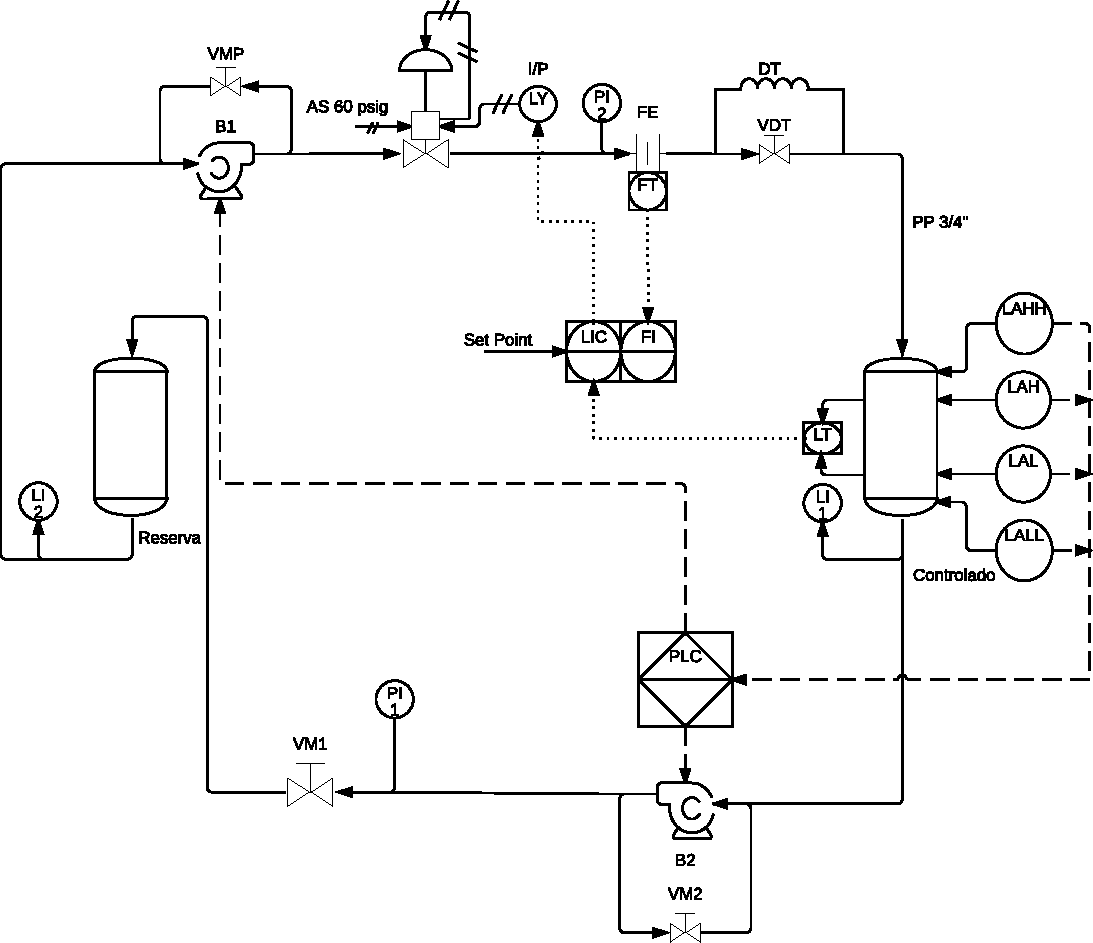
\includegraphics[width=.49\textwidth]
{Sections/2-DisenoEnsamblado/Images/pyid60-1.pdf}
	  \end{figure}
	\end{center}
}

\frame{
	\ifdebug
	\frametitle{Especificaciones vs Solución Propuesta\hfill{\color{red}
\emph{A}}}
	\else
	\frametitle{Especificaciones vs Solución Propuesta}
	\fi

	\textbf{Solución Propuesta}...
	\hspace{1cm}
	\textbf{Especificaciones}...
	
	
	\begin{columns}
		\begin{column}{0.4\textwidth}
		  \begin{center}
		    \begin{figure}[h!]
		      \centering
			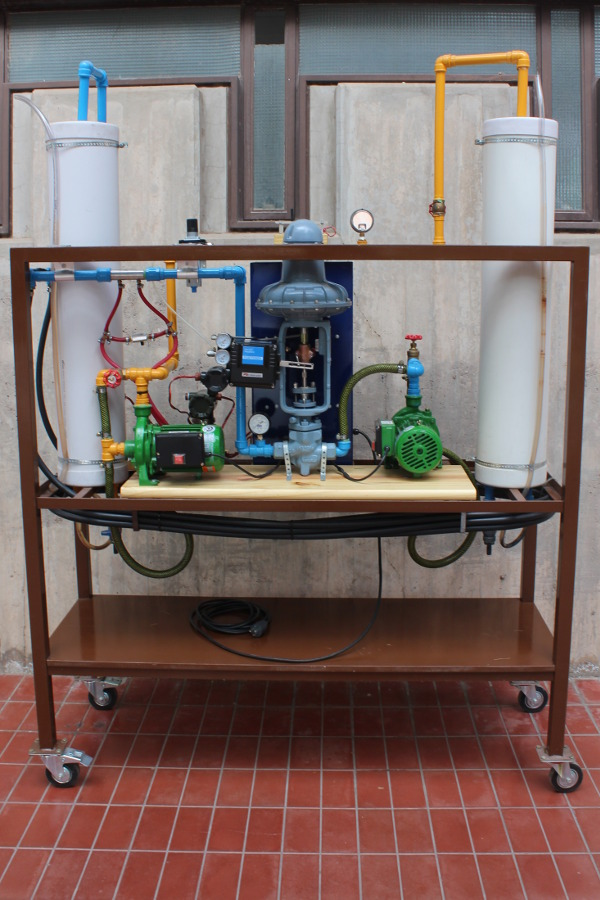
\includegraphics[width=\textwidth]
			 {Sections/1-Introduccion/images/IMG_5123.jpeg}
			\end{figure}
		   \end{center}
		\end{column}
		\begin{column}{0.5\textwidth}
		La planta debe:
			\begin{enumerate}
				\item Representar un ambiente industrial.
				\begin{itemize}
				 \item Procesos
				 \item Materiales
				\end{itemize}
				\item Cumplir un objetivo pedagógico.
				 \begin{itemize}
				  \item Verificar el funcionamiento 
del conjunto.
				  \item Documentar: Manual del usuario de la 
planta.
				 \end{itemize}
				\item Tener un costo inferior a una solución 
llave en mano.
			\end{enumerate}
		\end{column}
	\end{columns}
}

\frame{
	\ifdebug
	\frametitle{Análisis Económico\hfill{\color{red} \emph{A}}}
	\else
	\frametitle{Análisis Económico}
	\fi

	\begin{columns}
	  \centering
	 \begin{column}{0.3\textwidth}
	    \centering
	    \textbf{Cuál es el costo?}
	 \end{column}
	 
	 \begin{column}{0.3\textwidth}
	    \textbf{Plantas Similares:}
	    \begin{itemize}
	     \item Llave en mano.
	     \item Puerto de Bs.As.
	    \end{itemize}
	 \end{column}

	 \begin{column}{0.3\textwidth}
	    \begin{ukblock}
		\centering
		\textbf{16225\$} 
	    \end{ukblock}
	    \begin{itblock}
		\centering
		\textbf{\EUR{28403}}
	    \end{itblock}
	 \end{column}
	\end{columns}

	
	\vspace{-0.5cm}
	\begin{center}
%	 Las partes constitutivas de ambas plantas son elementos industriales
	 \end{center}
	\textbf{Donaciones:}
	\vspace{0.2cm}
	\begin{columns}[T]
	
	 \begin{column}{0.3\textwidth}
	    \begin{techintblock}
		\centering
		\textbf{5050\$}
	    \end{techintblock}
	    \footnotesize
	    \begin{itemize}
	     \item Electrobombas
	     \item PLC+PS+Mod. Analógico
	     \item DP Cell
	     \item Válvula de control
	    \end{itemize}
	 \end{column}
	 
	 \begin{column}{0.3\textwidth}
	    \begin{fingblock}
		\centering
		\textbf{2122\$}
	    \end{fingblock}
	    \footnotesize
	     \begin{itemize}
	      \item Estructura
	      \item Tuberías y Acc.
	      \item Material Eléctrico
	      \item Manómetros.
	     \end{itemize}
	 \end{column}

	 \begin{column}{0.3\textwidth}
	    \begin{puglesiblock}
		\centering
		\textbf{50\$}
	    \end{puglesiblock}
	    \footnotesize
	    \begin{itemize}
	     \item Placa Orificio
	    \end{itemize}

	 \end{column}

	\end{columns}
	
}

\frame{
	\ifdebug
	\frametitle{División del trabajo\hfill{\color{red} \emph{A}}}
	\else
	\frametitle{División del trabajo}
	\fi

	\textbf{Idea:} ...
	\vspace{0.25cm}
	\begin{center}

		Lorem ipsum dolor sit amet, consectetur adipiscing elit.
		Donec viverra cursus pellentesque. In et mattis augue.
		Dorbi ut velit a ante ultrices ornare in id nisl.

		\vspace{0.5cm}

		Pellentesque sollicitudin bibendum leo lobortis sagittis.
		Fusce eu purus vel mauris vestibulum mattis.
	\end{center}
}

\begin{frame}
	\ifdebug
	\frametitle{Outline\hfill{\color{red} \emph{A}}}
	\else
	\frametitle{Outline}
	\fi

    \tableofcontents
\end{frame}
